\documentclass[11pt,a4paper]{report}
\usepackage[utf8]{inputenc}
\usepackage[french]{babel}
\usepackage[T1]{fontenc}
\usepackage{amsmath}
\usepackage{amsfonts}
\usepackage{amssymb}
\usepackage{listings}
\usepackage{caption}
\usepackage{alltt}
%\usepackage{picins}
\usepackage{color}
\usepackage[left=2cm,right=2cm,top=2cm,bottom=2cm]{geometry}
\usepackage{hyperref}
\usepackage{graphicx}
\author{Adonis Najimi, Yvette Cheng, Taha Elleuch et Vicky Dincher}
\title{Rapport de projet d'Intergiciels} 
\date{27 Janvier 2016}

\renewcommand{\thesection}{\arabic{section}}
%\setcounter{tocdepth}{3}
\begin{document}
\maketitle
%\tableofcontents
\newpage
 
\section*{Introduction}

L'idée de notre projet, a été de réaliser un site web, permettant à des joueurs de posséder leurs Tamagochis (qui s'apparenteraient à des animaux de compagnie). Ces Tamagochis peuvent être nourris, nettoyés, et ainsi, chaque joueur voient leurs Tamagochis évoluer selon les objets ou les capacités qu'ils leur donnent. \\
Nous avions également décidé d'implémenter un jeu du type course entre plusieurs joueurs. Ainsi, chaque joueur pourrait rejoindre une salle de jeu, et jouer contre d'autres joueurs en ligne avec l'un de ses Tamagochis préalablement choisi. \\
L'idée principale était que chaque joueur puisse jouer avec son téléphone de la même manière qu'on joue avec une manette.

\section{Mise en place du modèle}

Les classes du modèle de notre projet ont été implémentées dans le dossier \texttt{model/} de notre application, les Joueurs, Tamagochis et Objets étant des entités. \\
Deux façades ont été réalisées, celle des joueurs et celle des Tamagochis. Elles permettent de gérer les différentes associations qui peuvent se faire entre les entités, ainsi que certaines requêtes, comme par exemple, trouver un joueur grâce à son adresse email (utile pour la connexion d'un joueur déjà enregistré).

\begin{figure}[h!]
\begin{center}
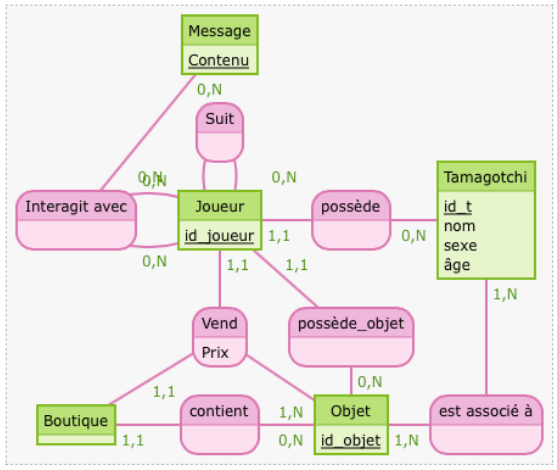
\includegraphics[scale=0.5]{Schemabdd.png}
\end{center}
\end{figure}

Le modèle prévu à la base a été réduit, faute de temps. Nous n'avons pu gérer les relations entre les joueurs (les demandes d'amis) ou les objets et la boutique.
\end{document}